\chapter{Funktionale Anforderungen}

\section{\gls{App}}
\begin{enumerate}
\renewcommand{\labelenumi}{\textbf{\theenumi}}
\renewcommand{\theenumi}{FA\arabic{enumi}0}
\setcounter{enumi}{99}
\item \textbf{Anzeigen der Einlog-Ansicht} \hfill \\
Öffnet der Benutzer die \gls{App} und sind keine Nutzerdaten gespeichert, so gelangt er in die Einlog-Ansicht. Dort kann er sich einloggen. Das Erstellen von Benutzeraccounts ist hier \textbf{nicht} möglich.

\item \label{fa:Anmeldedaten}\textbf{Anmeldedaten} \hfill \\
Anmeldedaten bestehen aus der E-Mai-Adresse und dem Passwort des Nutzers. Anemeldedaten werden lokal auf dem Gerät abgespeichert. Das Passwort wird als \gls{Hash-Code} gespeichert.

\item \textbf{Einloggen in die \gls{App}} \hfill \\
Beim Appstart muss sich der Nutzer zunächst einloggen. Zum Einloggen in die \gls{App} müssen die Anmeldedaten~\eqref{fa:Anmeldedaten} des Nutzers korrekt in die entsprechenden Felder eingetragen sein. Nur verifizierte Nutzer ~\eqref{fa:erstellAcc}) können sich einloggen. Beim Einloggen werden Nutzername und Passwort durch eine Serveranfrage geprüft. Bei falschen Eingaben oder wenn der Nutzer seinen Account nicht verifiziert hat erhält der Nutzer eine Fehlermeldung. Hat sich ein Nutzer bereits zuvor angemeldet, ohne sich wieder abzumelden, gelangt der Nutzer direkt zur Kamera-Ansicht. Die überprüfung der gespeicherten Anmeldedaten erfolgt dann erst beim Hochladen verschlüsselter Videodaten auf den Server~\eqref{fa:vidHochladen}.

\item \label{fa:logOut}\textbf{Ausloggen von einem Benutzeraccount} \hfill \\
Klickt ein Benutzer im Menü auf ``ausloggen'', so wird er auf die Einlog-Ansicht zurückgeleitet und seine Anemldedaten~\eqref{fa:Anmeldedaten} vom Gerät gelöscht.

\item \label{fa:Beobachtungsmodus}\textbf{Ausführen des Beobachtungsmodus} \hfill \\
Die Kamera kann sich bei aktiver Kamera in zwei Modi befinden: Im Beobachtungsmodus oder im Aufnahmemodus~\eqref{fa:Aufnahmemodus}.
Im Beobachtungsmodus werden Kamerabilder nicht \glslink{persistieren}{persistiert} sondern nur der \gls{Ringpuffer}~\eqref{fa:Ringpuffer} beschrieben. Die \gls{G-Sensor}-Daten werden ausgewertet und es wird auf einen charakteristischen Ausschlag des G-Sensors gewartet.

\item \label{fa:Statussymbol}\textbf{Anzeigen des Statussymbols} \hfill \\
Der aktuelle Kameramodus wird dem Nutzer durche ein blinkendes Statussymbol am Bildschirmrand visualisiert. Im Beobachtungsmodus hat es eine grüne Farbe, im Aufnahmemodus hat es eine rote Farbe.

\item \label{fa:camStart}\textbf{Starten der Beobachtung} \hfill \\
Wird die Kamera-Ansicht gestartet, befindet sich die Kamera sofort im Beobachtungsmodus. Nun wird der \gls{Ringpuffer}~\eqref{fa:Ringpuffer} beschrieben.

\item \textbf{Stoppen der Beobachtung} \hfill \\
Wenn der Benutzer die Kamera-Ansicht während der Beobachtung verlässt, oder die \gls{App} schließt, wird die Beobachtung automatisch beendet.

\item \label{fa:automUebergang}\textbf{Durch \gls{G-Sensor} ausgelöster Übergang in den Aufnahmemodus} \hfill \\
Werden die in ~\eqref{na:GSensfront} bis ~\eqref{na:GSensvert} definierten Richtwerte des G-Sensors überschritten, während die \gls{App} die Kamera-Ansicht anzeigt, geht die Kamera in den Aufnahmemodus über~\eqref{fa:Aufnahmemodus}. 

\item \label{fa:manUebergang}\textbf{Manueller Übergang in den Aufnahmemodus} \hfill \\
Befindet sich die Kamera im Beobachtungsmodus~\eqref{fa:Beobachtungsmodus} geht sie nach doppeltem Tippen auf die Vorschaufläche der Kamera-Ansicht in den Aufnahmemodus über.

\item \label{fa:Aufnahmemodus}\textbf{Ausführen des Aufnahmemodus} \hfill \\
Die Kamera kann sich bei aktiver Kamera in zwei Modi befinden: Im Beobachtungsmodus~\eqref{fa:Beobachtungsmodus} oder im Aufnahmemodus.
Im Aufnahmemodus wird der \gls{Ringpuffer}~\eqref{fa:Ringpuffer} für weitere 30 Sekunden beschrieben und anschließend dessen Inhalt im Hintergrund verschlüsselt~\eqref{fa:Verschluesselung} und \glslink{persistieren}{persistiert}. Die \gls{G-Sensor}-Daten sowie Nutzereingaben werden während sich die Kamera im Aufnahmemodus befindet ignoriert. Die Messwerte des G-Sensors, Zeit und Auslöseart(~\eqref{fa:manUebergang}, ~\eqref{fa:automUebergang}) werden in die \gls{Metadaten} der Videodatei geschrieben. Nach Ablauf der erwähnten 30 Sekunden wechselt die Kamera wieder zurück in den Beobachtungsmodus~\eqref{fa:Beobachtungsmodus}.

\item \label{fa:Ringpuffer}\textbf{\gls{Ringpuffer} beschreiben} \hfill \\
Der Ringpuffer stellt einen temporären Speicher dar, in den die Bilder der Kamera unverschlüsselt geschrieben werden. Dabei verhält er sich wie eine Warteschlange und fasst eine Minute Videomaterial, die Tonspur wird verworfen. Die später \glslink{persistieren}{persistierte} Videodatei soll 30 Sekunden vor dem Übergang der Kamera in den Aufnahmemodus und 30 Sekunden nach dem Übergang enthalten, wobei sich der Übergang in der Mitte des Videos befinden soll.

\item \label{fa:Verschluesselung}\textbf{Verschlüsseln eines Videos} \hfill \\
Videodaten werden durch das unter Kaptiel 9.4 defininierte hybrides Verschlüsselungsverfahren verschlüsselt.

\item \begin{minipage}[t]{\linewidth} 
\textbf{Anzeigen des Menüs} \hfill \\
	\begin{wrapfigure}{r}{0.4\linewidth}
		\vspace{-70pt}
  		\begin{center}
   			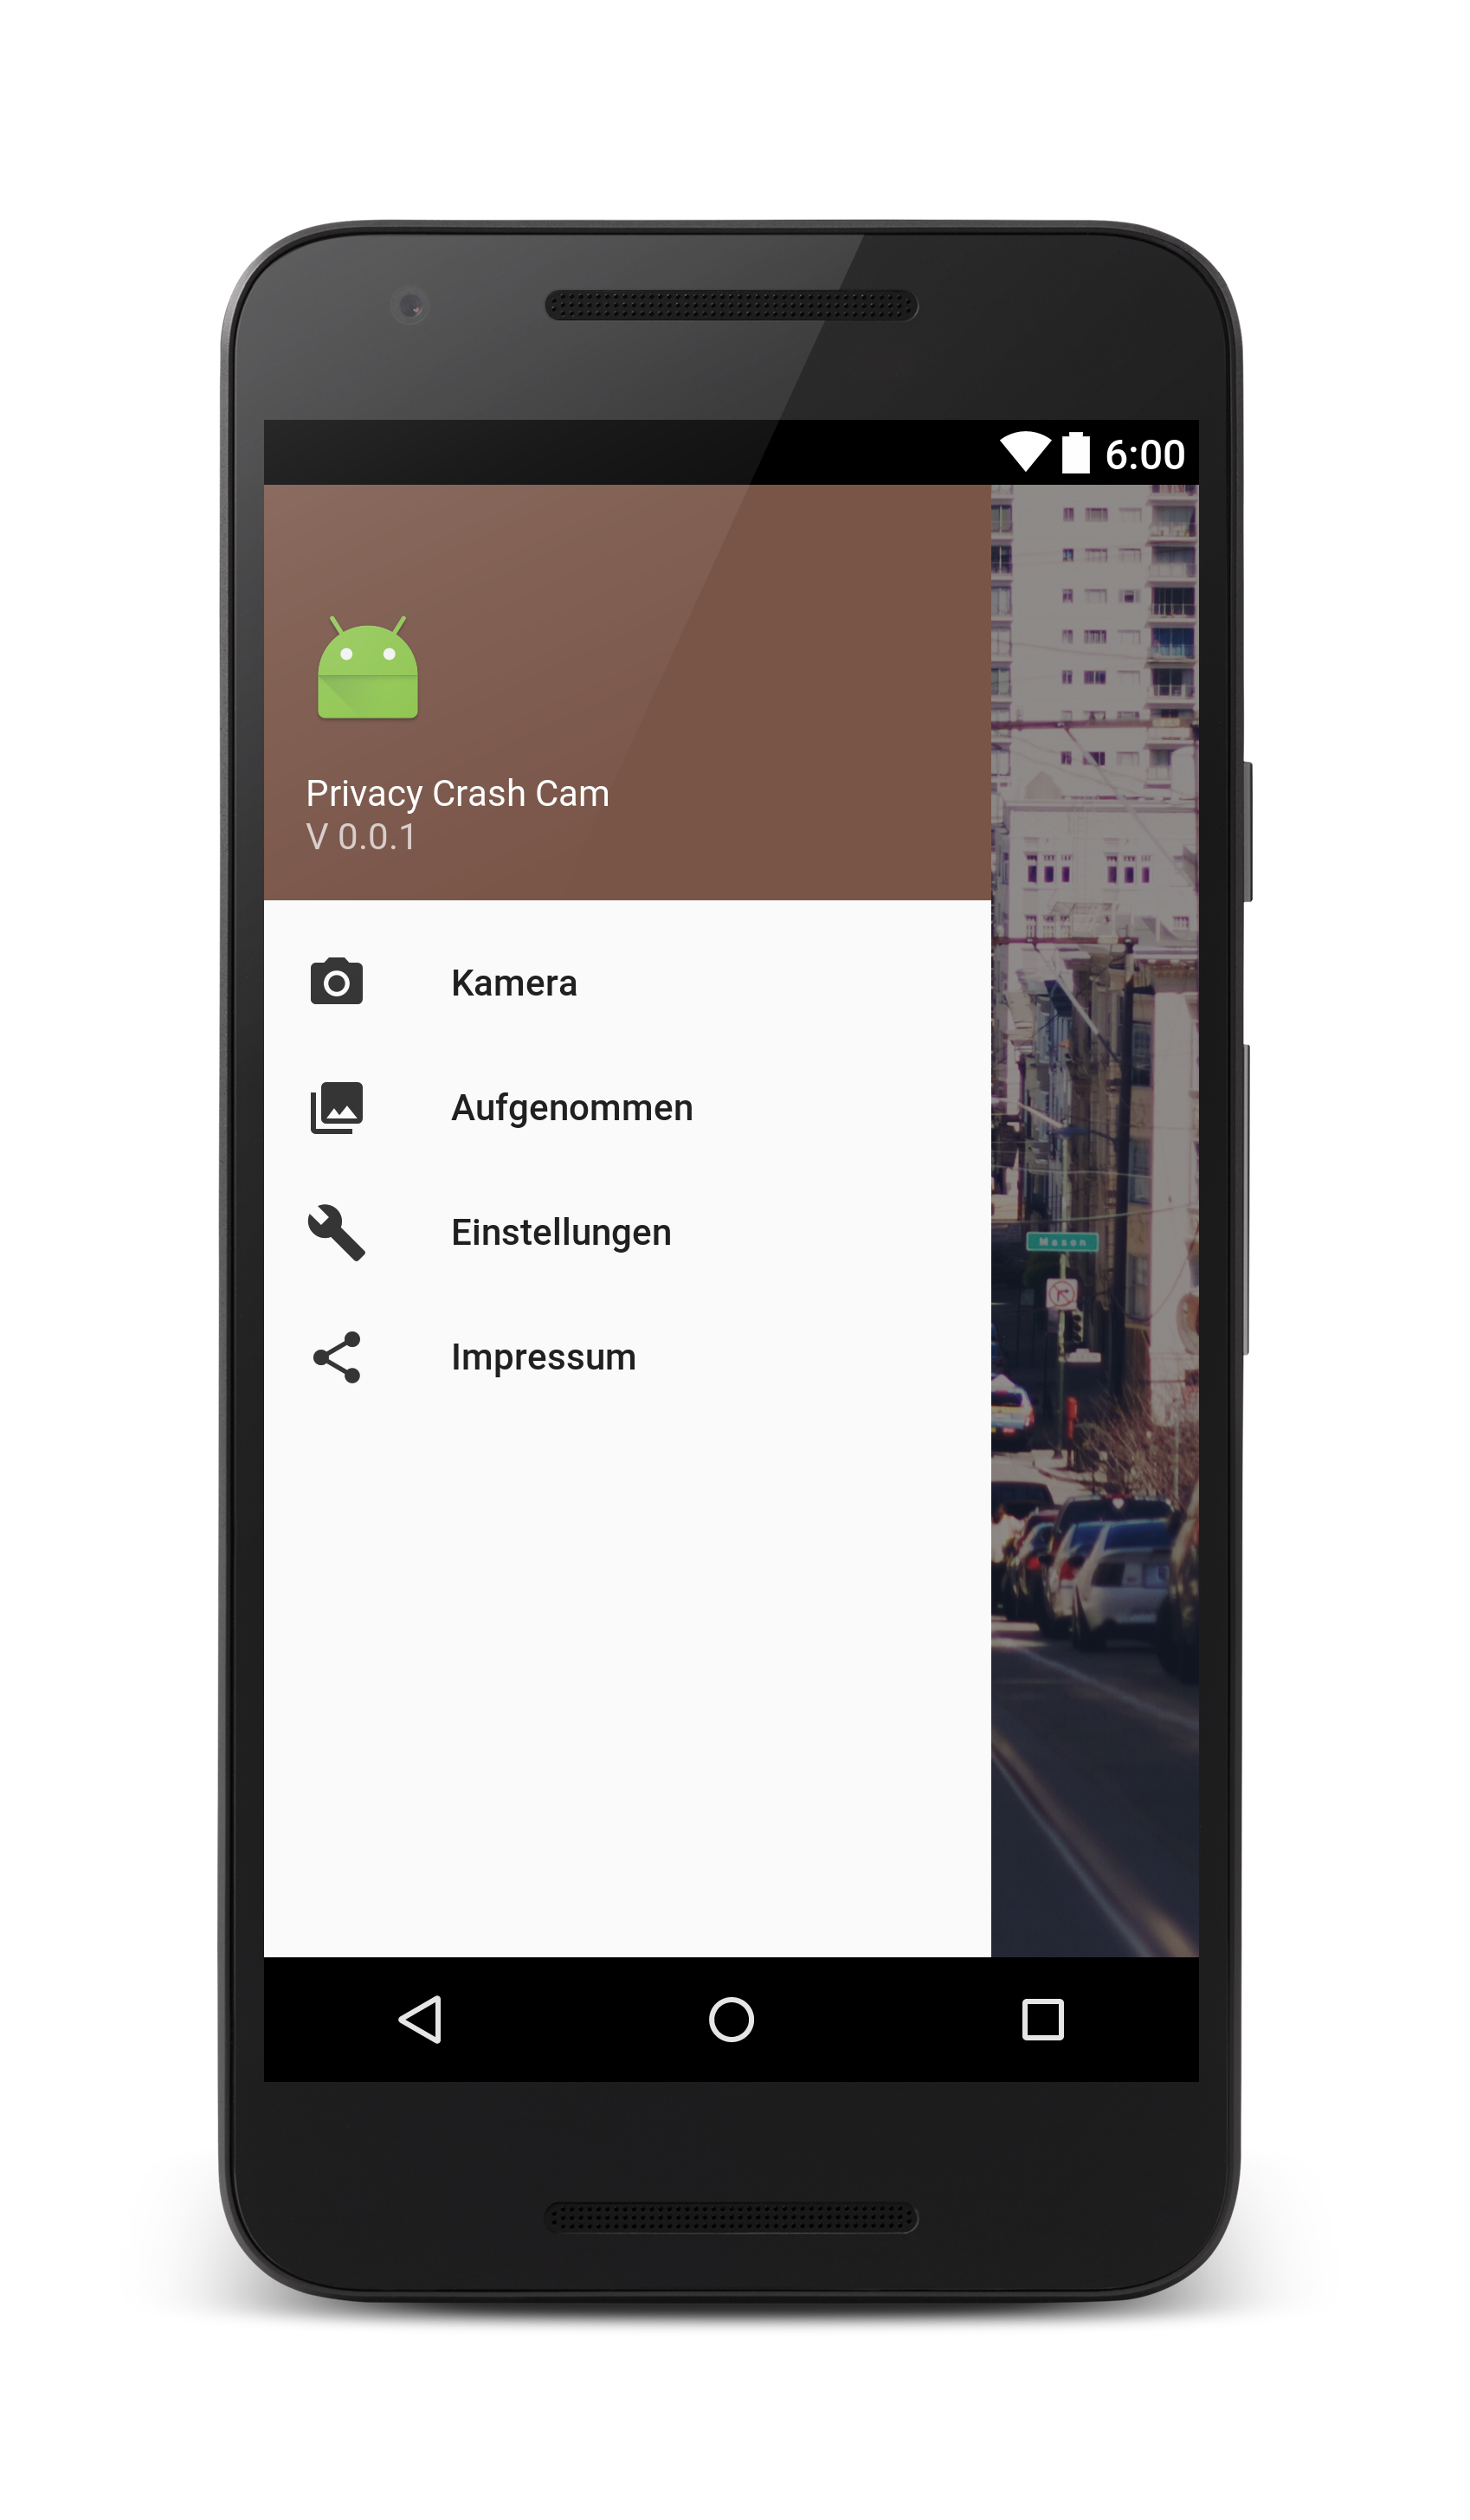
\includegraphics[width=0.4\textwidth]{subtopicsFuncspec/Res/Mockups/Portrait_camera_view_menu_phone.png}
  		\end{center}
  		\vspace{-20pt}
  		\vspace{-10pt}
	\end{wrapfigure}
Drückt der Benutzer den ``Menü-Button'' in der oberen linken Ecke des Bildschirms, so öffnet sich das Menü. befindet sich die Kamera im Beobachtungsmodus, während das Menü geöffnet wird, wird die Aufnahme nicht gestoppt. In dem Menü hat der Benutzer die Möglichkeit zwischen den verschiedenen \gls{App}-Ansichten Video-Ansicht~\eqref{fa:vidAnsicht}, Einstellungs-Ansicht~\eqref{fa:einstAnsicht} und Impressum-Ansicht~\eqref{fa:imprAnsicht} oder sich auszuloggen~\eqref{fa:logOut}.

\item \label{fa:vidAnsicht}\textbf{Anzeigen der Liste der \glslink{persistieren}{persistierten} Videos} \hfill \\
Wählt der Benutzer im Menü die Option ``Aufgenommen'', so gelangt er zu einer Ansicht, in dem ihm seine persistierten Videos chronologisch aufgelistet werden. Der Nutzer kann Videos hochladen~\eqref{fa:vidHochladen}, löschen~\eqref{fa:vidLöschen}, oder Videoinformationen einsehen~\eqref{fa:metaVerschlVid}.
\end{minipage}

\item \label{fa:vidHochladen}\textbf{Hochladen von gespeicherten Videos} \hfill \\
Klickt der Nutzer auf den ``Upload-Button'', wird ein Dialog aufgerufen, in dem der Nutzer darauf hingewiesen wird, dass mobile Daten anfallen werden. Wenn der Benutzer akzeptiert, schickt die \gls{App} eine Anfrage an den Server. Dieser beantwortet die Anfrage falls Ressourcen verfügbar und die auf dem Gerät gespeicherten Anmeldedaten des Nutzers korrekt sind und erlaubt den Upload. In jedem Fall wird dem Nutzer eine Erfolgs- bzw. Misserfolgsnachricht gezeigt. Durch Tippen auf diese kann er zur Liste seiner Videos~\eqref{fa:vidAnsicht} gelangen.

\item \label{fa:vidLöschen}\textbf{Löschen von gespeicherten Videos} \hfill \\
Klickt der Benutzer auf das ``Löschen-Symbol'', so wird ein Bestätigungsdialog~\eqref{fa:vidLöschenDialog} geöffnet. Falls der Benutzer bestätigt wird das Video aus der Liste seiner \glslink{persistieren}{persistierten} Videos entfernt und vom Gerät gelöscht. Bricht der Benutzer den Dialog ab bleibt er in der Listenansicht seiner Videos.

\item \label{fa:vidLöschenDialog}\textbf{Anzeigen einer Benachrichtigung zum Löschen von Videos} \hfill \\
Beim Einloggen und bei jedem Appstart wird geprüft, ob \glslink{persistieren}{persistierte} Videos bereits seit über 4 Wochen auf seinem Gerät gespeichert sind. Ist dies so wird ihm ein Dialog angezeigt, der ihn auf diesen Umstand hinweist. Dort wird ihm angeboten, das Video zu löschen~\eqref{fa:vidLöschen}. Bricht er den Dialog ab, gelangt er wie üblich in die Kamera-Ansicht~\eqref{fa:camStart}.

\item \label{fa:metaVerschlVid}
\textbf{Einsehen von Video-Daten der verschlüsselten Videos} \hfill \\
\begin{minipage}[t]{\linewidth}
	\begin{wrapfigure}{r}{0.4\linewidth}
		\vspace{-35pt}
  		\begin{center}
   			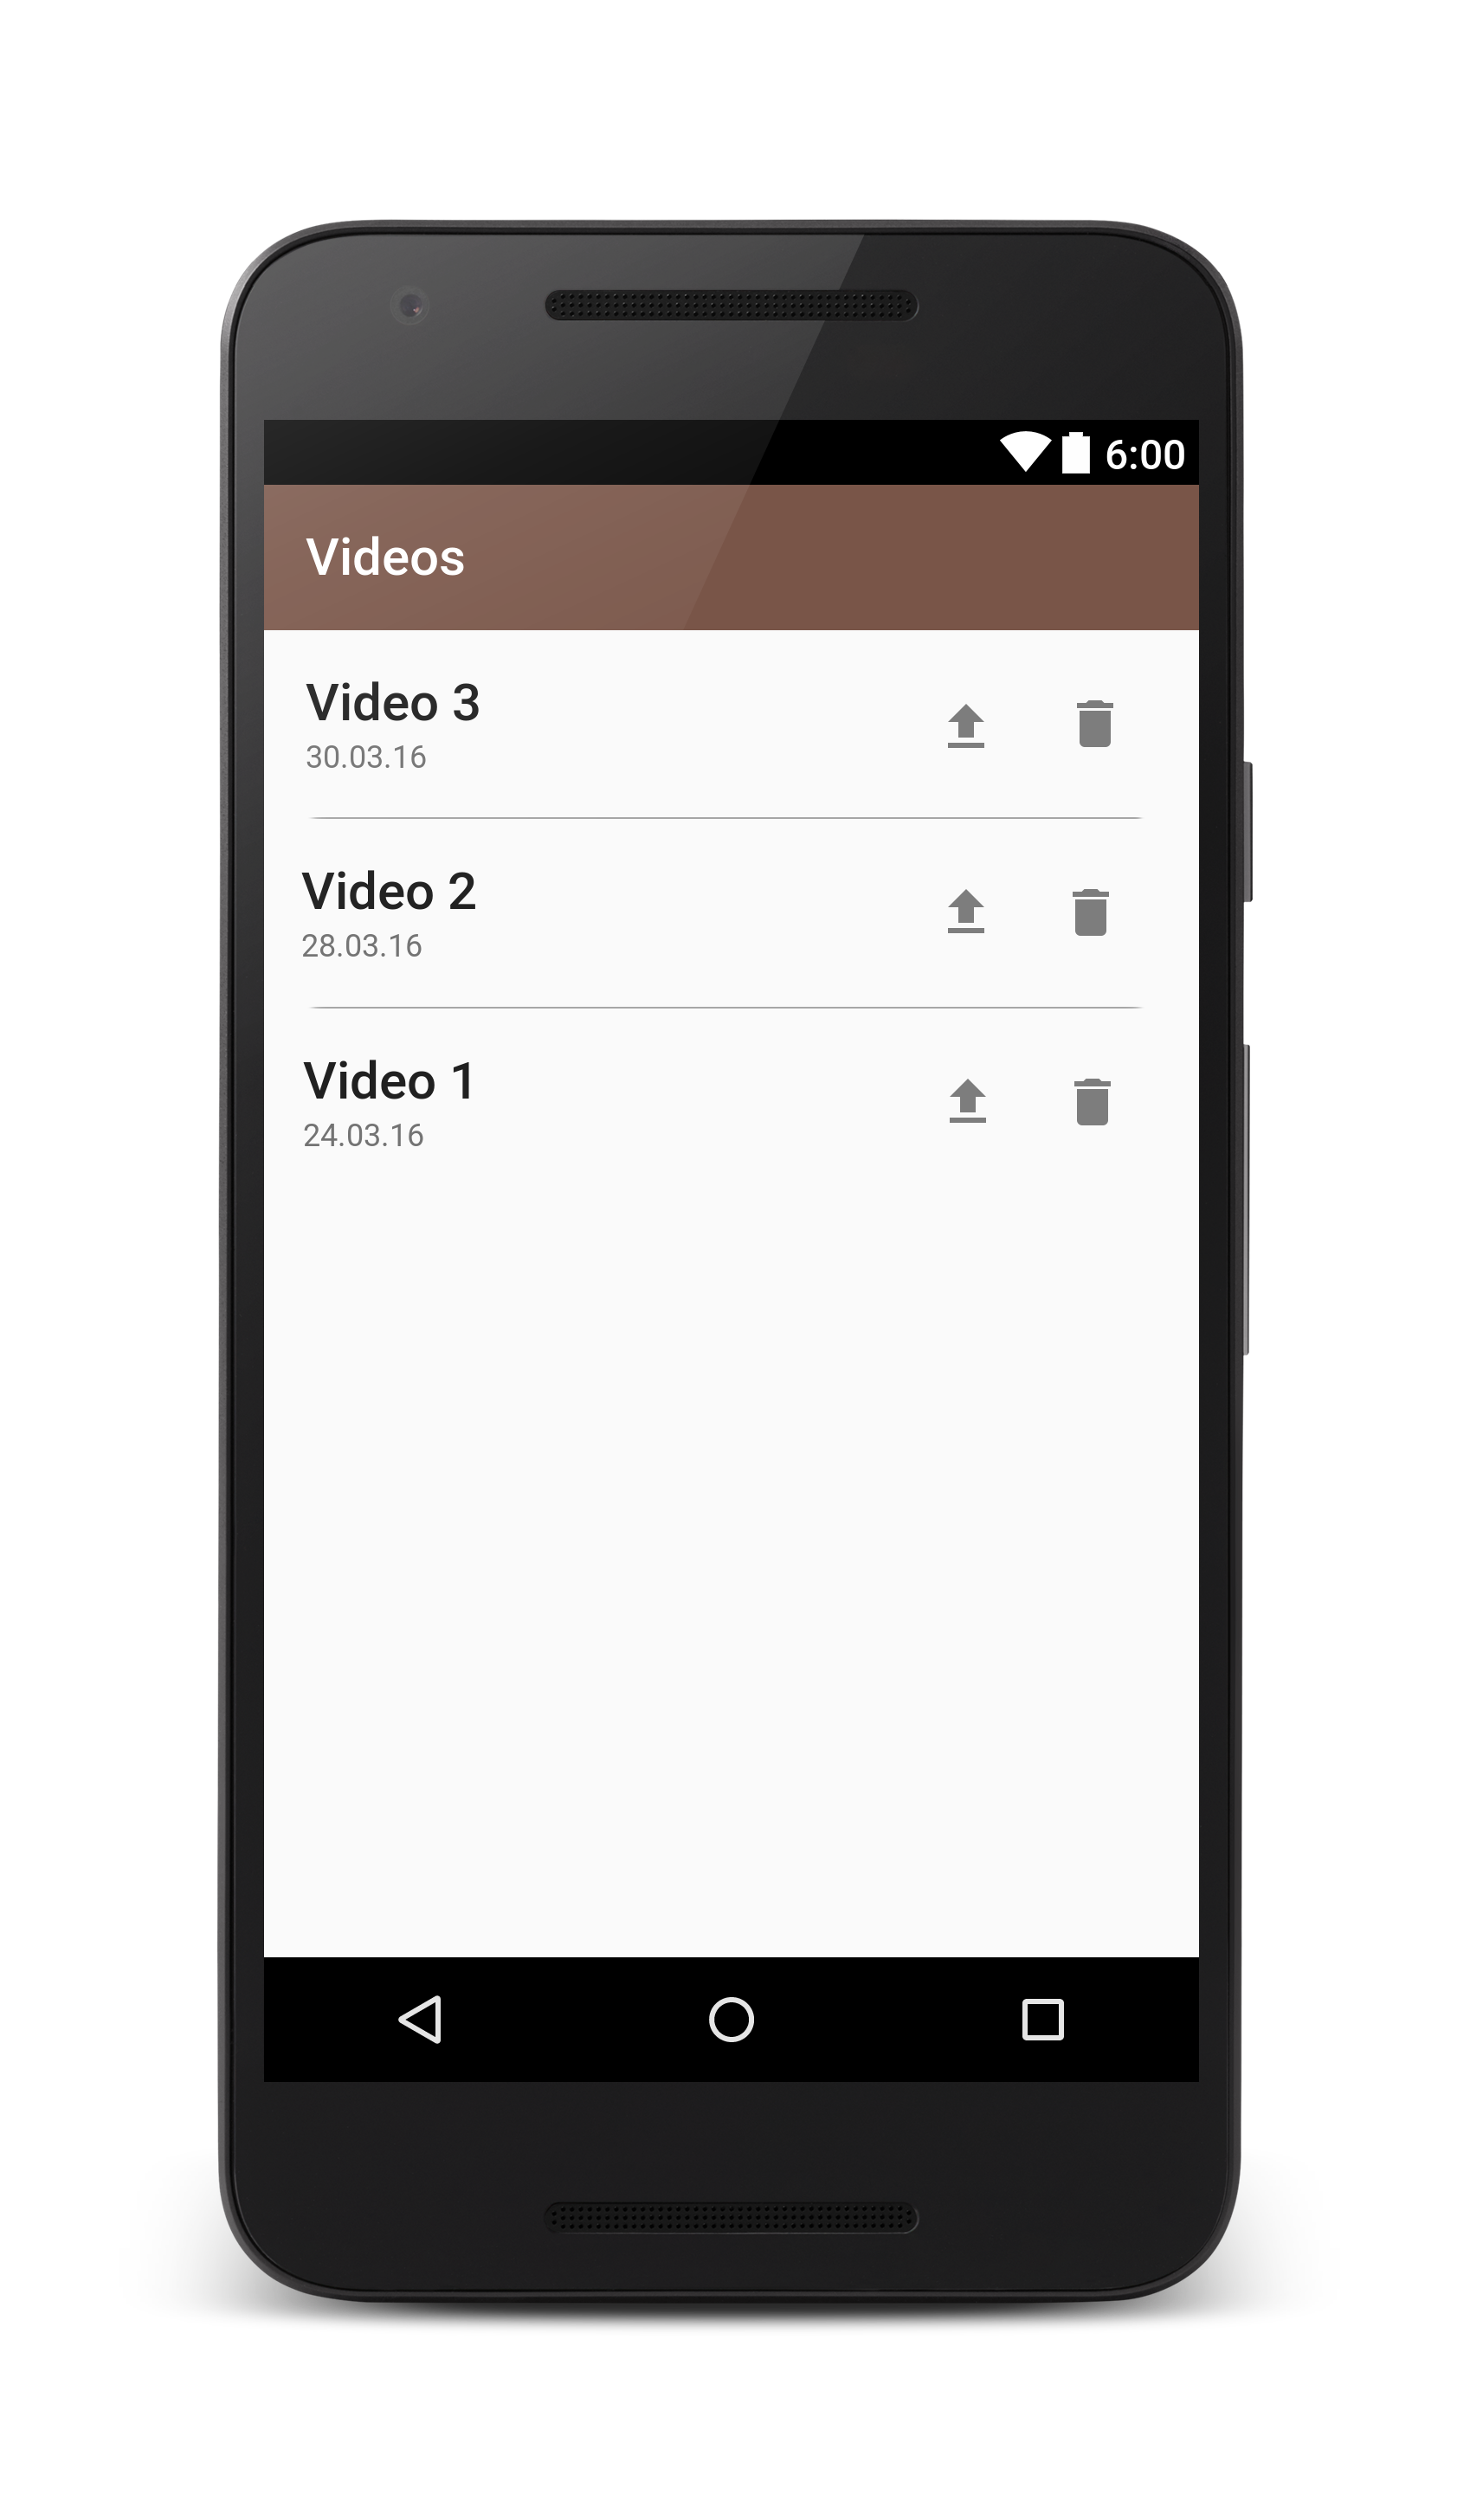
\includegraphics[width=0.4\textwidth]{subtopicsFuncspec/Res/Mockups/Videos_list1_phone.png}
  		\end{center}
  		\vspace{-20pt}
  		\vspace{-10pt}
	\end{wrapfigure}
Klickt der Benutzer lange auf ein Video wird ein Fenster geöffnet, dass dem Benutzer die Video-\gls{Metadaten} (Erstellungsdatum, Größe, Auflösung, Dauer, Auslöseart, \gls{G-Sensor}-Daten) als Dialog anzeigt. Schließt der Nutzer den Dialog, kehrt er zu der Liste seiner Videos~\eqref{fa:vidAnsicht} zurück.

\item \label{fa:einstAnsicht}\textbf{Anzeigen der Einstellungen} \hfill \\
Wählt der Benutzer im Menü die Option ``Einstellungen'', so werden dem Nutzer die Standardeinstellungen angezeigt (Auflösung, Bildwiederholrate, Größe \gls{Ringpuffer}) angezeigt.

\item \label{fa:imprAnsicht}\textbf{Anzeigen rechtlicher Informationen} \hfill \\
Wählt der Benutzer im Menü die Option ``Impressum'', gelangt er zur Impressums-Ansicht. Von dort kann er sich das Impressum~\eqref{fa:imprAnzeigen} und die Datenschutzerklärung~\eqref{fa:datenschAnzeigen} anzeigen lassen.
\end{minipage}

\item \label{fa:imprAnzeigen}\textbf{Anzeigen des Impressums} \hfill \\
Wählt der Benutzer ``Impressum'' auf der Impressum-Ansicht, wird ein Dialog angezeigt, der das Impressum anzeigt.

\item  \label{fa:datenschAnzeigen}\textbf{Anzeigen der Datenschutzerklärung} \hfill \\
Wählt der Benutzer ``Datenschutzerklärung'' auf der Impressum-Ansicht, wird ein Dialog angezeigt, der die Datenschutzerklärung anzeigt.

\end{enumerate}

\section{\gls{Web-Dienst}}
\begin{enumerate}
\renewcommand{\labelenumi}{\textbf{\theenumi}}
\renewcommand{\theenumi}{FA\arabic{enumi}0}
\setcounter{enumi}{199}

\item  \textbf{Empfangen eines Videos von der \gls{App}} \hfill \\
Bekommt der \gls{Web-Dienst} eine Anfrage von der App ein Video hochzuladen, so überprüft er zunächst, ob er die Anfrage bearbeiten kann, oder ob bereits zu viele andere Anfragen gestellt wurden ~\eqref{na:paralleleZugriffe}. Ist dies nicht der Fall, so speichert er das Video temporär~\eqref{fa:entschVideo} und beginnt die Anonymisierung~\eqref{fa:anonymVideo}.

\item  \label{fa:entschVideo}\textbf{Entschlüsseln eines empfangenen Videos} \hfill \\
Bevor der \gls{Web-Dienst} die Bearbeitung des Videos beginnt, entschlüsselt er das empfangene verschlüsselte Video. Hierbei wird das unter Kaptiel 9.4 defininierte Verschlüsselungsverfahren angewandt. Das entschlüsselte Video wird lokal temporär gespeichert.

\item \label{fa:mailSenden}\textbf{Versenden einer Bestätigungsmail} \hfill \\
Hat ein Benutzer das Anmeldeformular ~\eqref{fa:erstellAcc} ausgefüllt, so versendet der \gls{Web-Dienst} eine Bestätigungsmail. Klickt der Benutzer auf den dort vorhanden Bestätigungslink so wird der Account verifiziert und auf dem Server gespeichert ~\eqref{fa:accSpeichern}.

\item \label{fa:accSpeichern}\textbf{Speichern eines Accounts} \hfill \\
Wenn ein Account verifiziert wurde, werden seine Daten auf dem Server gespeichert. Passwörter werden ausschließlich als \gls{Hash-Code} abgelegt.

\item \label{fa:accLöschen}\textbf{Löschen eines Accounts} \hfill \\
Wenn der Nutzer seinen Account löschen will werden zunächst alle, von ihm hochgeladenen Videos vom Server gelöscht. Wird gerade ein Video von dem anonymisiert, so wird dieses nach der Anonymisierung nicht gespeichert. Danach werden die Accountdaten des Nutzers gelöscht.

\item  \label{fa:relBildbereiche}\textbf{Identifizieren der relevanten Bildbereiche} \hfill \\
Der \gls{Web-Dienst} nimmt das entschlüsselte Video und lässt einen Bildfilter über das Video laufen, der die für die Anonymisierung relevanten Bildbereiche (Gesichter, Nummernschilder, etc.) erkennt. Die so ermittelteten Bereiche werden in einer Bitmaske gespeichert.

\item  \label{fa:anonymVideo}\textbf{Anonymisierung des Videos} \hfill \\
Der \gls{Web-Dienst} nimmt die in ~\eqref{fa:relBildbereiche} erstellte Bitmaske um die dort makierten relevanten Bildbereiche mithilfe eines Anonymisierungsfilters zu \gls{anonymisieren}.

\item \label{fa:speichVideo}\textbf{Abspeichern eines \glslink{anonymisieren}{anonymisierten} Videos} \hfill \\
Nachdem das Video anonymisiert wurde, wird es lokal auf dem Server gespeichert und alle temporären Dateien gelöscht. Das gespeicherte Video wird der Videoverwaltung hinzugefügt damit es vom Benutzer eingesehen und bearbeitet werden kann. Wenn ein Benutzer die maximale Anzahl Videos pro Account ~\eqref{na:VideoKap} überschreitet, wir automatisch das älteste Video des Accounts auf dem Server gelöscht.
\end{enumerate}

\textbf{TODO Account löschen ist eine Funktion des Web-Diestes die vom Interface aufgerufen wird; Passwort ändern und Email ändern auch, diese Fktnen. fehlen aber ganz; Unterscheidung ob Nutzer bereits wo anders eingeloggt ist ist aufwendig und nicht wirklich praktikabel, sollten wir raus nehmen; zu Accounterstellung gehört auch speicherung des PW als Hash }

\section{\gls{Web-Interface}}
\begin{enumerate}
\renewcommand{\labelenumi}{\textbf{\theenumi}}
\renewcommand{\theenumi}{FA\arabic{enumi}0}
\setcounter{enumi}{299}
\item \label{fa:loginWeb} \textbf{Anzeigen der Einlog-Ansicht} \hfill \\
Ruft der Nutzer die Privacy-Crash-Cam-Webseite auf, so gelangt er zu der Einlog-Ansicht. Dort kann sich der Benutzer anmelden ~\eqref{fa:weblogIn} oder sich registrieren ~\eqref{fa:erstellAcc}.

\item \label{fa:erstellAcc}\textbf{Erstellen eines Benutzeraccount} \hfill \\
Klickt der Benutzer auf "'Account erstellen"' so öffnet sich der Registrierungsdialog. Dort wird der Nutzer gebeten einen einzigartigen Benutzername und eine \gls{E-Mail} Adresse angegeben. Zudem muss er ein Passwort auswählen und bestätigen. Klickt der Nutzer auf "'Registrierung abschließen"' werden die Eingaben überprüft. Schlägt dies fehl bleibt der Benutzer in dem Registrierungsdialog. Nach dem Erstellen eines Benutzeraccounts sendet der Server eine Bestätigungsmail ~\eqref{fa:mailSenden}.

\item \label{fa:weblogIn}\textbf{Einloggen auf die Webseite} \hfill \\
Zum Einloggen auf die Webseite müssen Benutzername und Passwort korrekt in die entsprechenden Felder eingetragen sein. Nur verifizierte Nutzer ~\eqref{fa:mailSenden} können sich einloggen. Ist ein Nutzer bereits angemeldet, so muss er sich zuerst in der zweiten Web-Sitzung ausloggen, bevor er sich einloggen kann. Bei falschen Eingaben oder wenn der Nutzer bereits eingeloggt ist kehrt er zur Einlog-Ansicht zurück und erhält eine Fehlermeldung.

\item \textbf{Anzeigen der Menüleiste} \hfill \\
Befindet sich der Nutzer in einer anderen Ansicht als der Einlog-Ansicht, so befindet sich am linken Rand der Websteite die Menüleiste. Dort kann der Nutzer die Liste der \glslink{anonymisieren}{anonymisierten} Videos ~\eqref{fa:anonymVidAnzeigen}, seinen Account bearbeiten ~\eqref{fa:accBearb}, die Datenschutzerklärung einsehen ~\eqref{fa:datenschutzWeb}, das Impressum einsehen ~\eqref{fa:impressumWeb}, oder sich ausloggen ~\eqref{fa:weblogOut}.

\item \label{fa:anonymVidAnzeigen}\textbf{Anzeigen der Liste der \glslink{anonymisieren}{anonymisierten} Videos} \hfill \\
Hat sich ein Benutzer eingeloggt wird er automatisch auf diese Ansicht weitergeleitet. Hier werden die, von dem Nutzer hochgeladenen Videos chronologisch aufgelistet. Der Nutzer kann Videos herunterladen ~\eqref{fa:anonymVidherunt}, löschen ~\eqref{fa:anonymVidlösch}, ein Preview einsehen ~\eqref{fa:anonymVidprev}, oder die Videoinformationen einsehen ~\eqref{fa:anonymViddaten}.

\item \label{fa:anonymVidherunt}\textbf{Herunterladen von \glslink{anonymisieren}{anonymisierten} Videos} \hfill \\
Durch einen Klick wird eine Speicherdialog geöffnet. Nachdem der Nutzer einen Speicherort ausgewählt hat wird das Video heruntergeladen. Bricht der Benutzer den Dialog ab, bleibt er in der Listenansicht seiner Videos.

\item \label{fa:anonymVidlösch}\textbf{Löschen eines \glslink{anonymisieren}{anonymisierten} Videos} \hfill \\
Durch den Klick auf das "'Löschen-Symbol"' wird ein Bestätigungsdialog geöffnet. Falls der Benutzer, bestätigt wird das Video aus der Liste seiner hochgeladenen Videos entfernt und vom Server gelöscht. Bricht der Benutzer den Dialog ab, bleibt er in der Listenansicht seiner Videos.

\item \label{fa:anonymVidprev}\textbf{Vorschau eines \glslink{anonymisieren}{anonymisierten} Videos} \hfill \\
Klickt der Benutzer auf das "'Vorschau-Symbol"', so wird ein Fenster geöffnet, in dem der Nutzer ein Vorschau des anonymisierten Videos angezeigt wird.

\item \label{fa:anonymViddaten}\textbf{Einsehen von Video-Daten der \glslink{anonymisieren}{anonymisierten} Videos} \hfill \\
Klickt der Benutzer auf das "'Info-Symbol"', so wird ein Fenster geöffnet, dass dem Benutzer die Video-\gls{Metadaten} (Erstellungsdatum, Datum der Anonymisierung, Größe, Auflösung, Dauer) anzeigt.

\item \label{fa:accBearb}\textbf{Bearbeiten eines Benutzeraccounts} \hfill \\
Klickt ein Benutzer in der Menüleiste auf "'Account bearbeiten"', so wird ein Fenster geöffnet in, dem der Nutzer auswählen will ob er seine Accountdaten ändern, oder seinen Account löschen will.

\item \label{fa:accLöschenWeb}\textbf{Account Löschen} \hfill \\
Klickt der Benutzer in dem Fenster ~\eqref{fa:accBearb} auf "'Account Löschen"', so öffnet sich ein Bestätigungsdialog, in dem der Benutzer gefragt wird, ob er wirklich seinen Account löschen will. Bestätigt dieser, so gelangt er zu der Einlogansicht ~\eqref{fa:loginWeb} und sein Account wird gelöscht ~\eqref{fa:accLöschen}.

\item \label{fa:accDatBearb}\textbf{Accountdaten bearbeiten} \hfill \\
Klickt der Benutzer in dem Fenster ~\eqref{fa:accBearb} auf "'Accountdaten ändern"', so kann er sein Passwort ändern. Dies macht er, in dem er zunächst in ein Feld sein altes Passwort und danach in zwei Felder sein neues gewünschtes Passwort eingibt. Stimmt das alte Passwort und stimmen die zwei Felder für das neue Passwort überein, so werden die Daten auf dem Server entsprechend geändert.

\item \label{fa:impressumWeb} \textbf{Anzeigen des Impressums} \hfill \\
Klickt der Benutzer in der Menüleiste auf "'Impressum"', so wird eine Sicht geöffnet, in der der Nutzer das Impressum einsehen kann.

\item \label{fa:datenschutzWeb} \textbf{Anzeigen der Datenschutzerklärung} \hfill \\
Klickt der Benutzer in der Menüleiste auf "'Datenschutz"', so wird eine Sicht geöffnet, in der der Nutzer die Datenschutzerklärung und die AGB einsehen kann.

\item \label{fa:weblogOut}\textbf{Ausloggen von der Webseite} \hfill \\
Klickt ein Benutzer in der Menüleiste auf "'Ausloggen"' so wird er auf die Einlog-Ansicht zurückgeleitet. Schließt ein Nutzer die Webseite, so wird er automatisch ausgeloggt.

\end{enumerate}